
\chapter{Week 5 -- Implementation of Mathematical Models}

\section{Abstract}
This report presents the Matlab implementation of a dynamic battery model based on an equivalent circuit. A battery cell is first modelled as a voltage source with internal impedance. Subsequently, two RC elements in series with internal impedance are added. Temperature and SOC dependence of individual parameters is considered as well. The cell model was fully parameterized in the assignment. Equations governing the behaviour of the given model were implemented in Matlab code to facilitate simulation.


\section{Simple battery model}

The first implemented model considered only an ideal voltage source $U_{OC}$ with impedance $R_0$ in series. The only state is the state of charge (here given in percent rather than in the range $\left[0, 1\right]$. The flowing current $I$ is the model input and the voltage across battery terminals $U_{bat}$ is the only output. This model is is governed by the state space
\begin{equation}
\begin{split}
    \dot{SOC} &= -\eta \frac{1}{C} I, \\
    U_{bat} &= U_{OC} - I R_0.
\end{split}
\label{eq:5-simple}
\end{equation}

The model was simulated over a time interval of 500 seconds with results shown in Fig. \ref{fig:5-simple}. Since the battery has total capacity of 3 Ah and the discharging current averages to 1 A, simple calculation predicts decrease of SOC by roughly 4.6 \%. Since this prediction matches the simulation result, one can conclude that the simulation yields sane results.


\begin{figure}[hbtp]
    \centering
    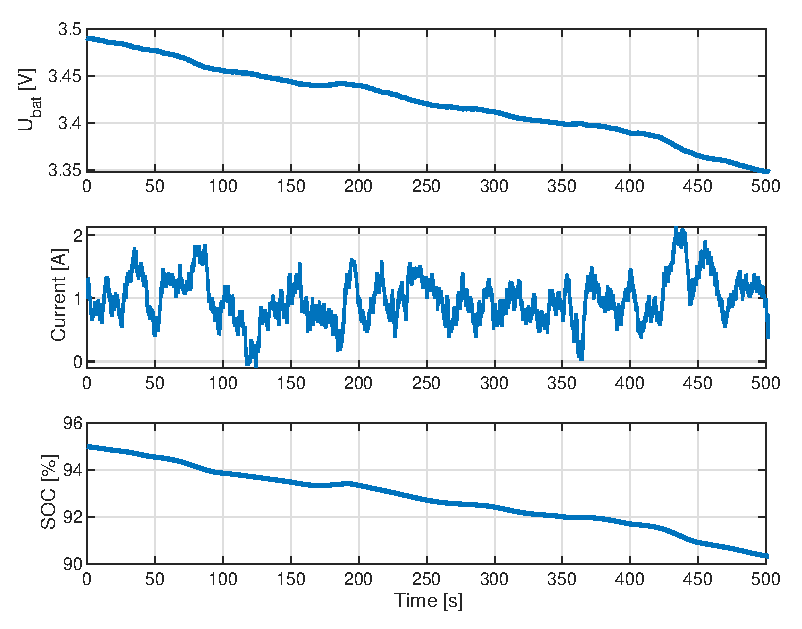
\includegraphics[width=0.8\textwidth]{figures/5/simple-everything.eps}
    \caption{Simulation results for simple battery model}
    \label{fig:5-simple}
\end{figure}

\section{Improved battery model}

The second implemented model added two RC elements with parameters $R_i$ and $C_i$ on top of the already considered simple model. This modification adds two states -- voltage drop $U_i$ across each RC element. This model is is governed by the state space
\begin{equation}
\begin{split}
    \dot{SOC} &= -\eta \frac{1}{C} I, \\
    \dot{U_1} &= -\frac{1}{R_1 C_1} U_1 + \frac{1}{C_1} I, \\
    \dot{U_2} &= -\frac{1}{R_2 C_2} U_2 + \frac{1}{C_2} I, \\
    \dot{SOC} &= -\eta \frac{1}{C} I, \\
    U_{bat} &= U_{OC} - I R_0 - U_1 - U_2.
\end{split}
\label{eq:5-complex}
\end{equation}


whose parameters are all temperature-dependent.

The model was simulated over a time interval of 500 seconds using temperature shown in Fig. \ref{fig:5-complex-temp} with results shown in Fig. \ref{fig:5-complex}. The discharged SOC again matches the expected value of roughly 5 \%. The terminal voltage $U_{bat}$ is generally lower than in case of the simple model since both models use identical values of the internal impedance $R_0$ and the improved model adds additional voltage drops. These observations prove the sanity of the implemented model and obtained results.

 Individual voltage drops across each RC element as well as the internal impedance $R_0$
 are shown in detail in Fig. \ref{fig:5-complex-RC}. Note how the voltage drop across $R_0$
 is negligible compared to the drop across each RC element -- $R_0$ is at least an order of magnitude lower than $R_1$ or $R_2$. This also explains why the terminal voltage $U_{bat}$ in Fig. \ref{fig:5-simple} is much smoother than $U_{bat}$ in Fig. \ref{fig:5-complex}.
 
\begin{figure}
    \centering
    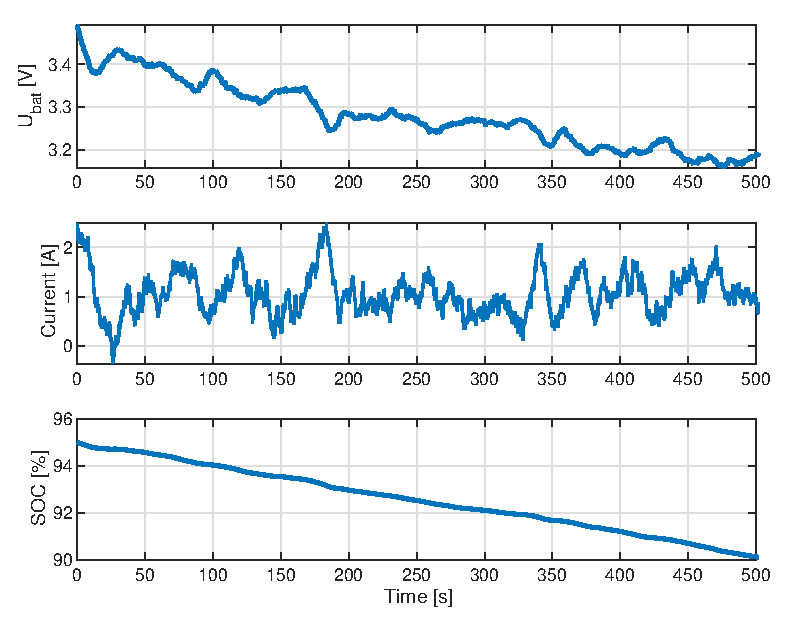
\includegraphics[width=0.8\textwidth]{figures/5/complex-everything.eps}
    \caption{Simulation results for improved battery model with two RC elements}
    \label{fig:5-complex}
\end{figure}

\begin{figure}
    \centering
    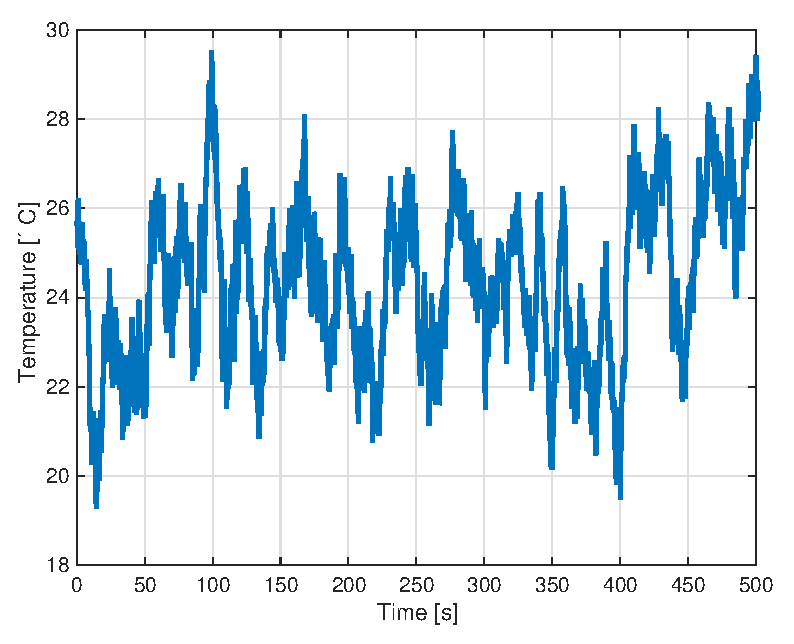
\includegraphics[width=0.6\textwidth]{figures/5/complex-Temp.eps}
    \caption{Temperature used for improved model simulation}
    \label{fig:5-complex-temp}
\end{figure}

\begin{figure}
    \centering
    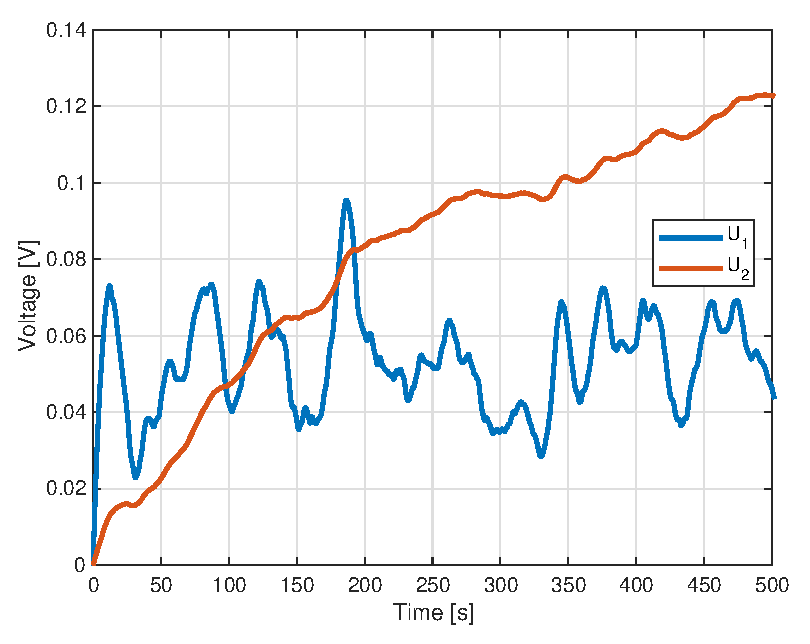
\includegraphics[width=0.6\textwidth]{figures/5/complex-U-RC.eps}
    \caption{Simulated voltage drops across each component of the improved model}
    \label{fig:5-complex-RC}
\end{figure}


